\chapter{Results}
For this dissertation, I apply three psychometric models to empirical data from two assessments designed to measure two different learning progressions (i.e., Force and Motion, and Earth and Solar System LPs). Recall that learning progressions are hypotheses about how student learning occur and each model provides empirical evidence that can be used to provide feedback on the LP assessments, and conjointly LP hypotheses. The goal of this analysis is to examine how each model provides information about learning progressions and assessments themselves, and to examine the viability of the models in the LP context. The primary goal of this chapter is to examine the FM LP data and present the results from basic categorization of students into LP levels. 

In this section,I describe the data used in the analyses, and I provide the results from the exploratory analysis of data. For the exploratory part, I examine the dimensionality of data. While it is not the main focus of the current dissertation, there is a question on LP assessments whether the data support multidimensional over unidimensional structure or vice versa given that these assessments were not explicitly developed to be modeled in either structure. For this first part, my examination of data aims to understand the data better for the later analyses and results. This is followed by an examination of the classification of students into LP levels from a modal analysis of the data in section. A fundamental argument in favor of taking a probabilistic approach to classifying students for diagnostic purposes is that such an approach offers more nuanced insights into a student's strengths and weaknesses than taking a more ad hoc or modal  approach, such as simply classifying a student as a function of his or her modal response. Thus, the results from modal approach are aimed to provide a basis for comparisons from the probabilistic models that I use in this dissertation to examine whether there is practical reasons to use more complicated models. That is, I will be able to examine the differences of the inferences made based on the modal approach with the classifications made using three probabilistic models. This chapter ends with a summary of the findings from exploratory analysis of data and results of student placement into the LP levels based on their modal selection of item options related to LP levels. The placement of students into the LP levels is done by counting the most frequent option they chose where each option is connected to a LP level.  
\section{\em Data}
The data used for this study originally included 16 Forces and Motion (FM) OMC items that were administered to a sample of 1,088 high school students at six schools in rural and suburban Iowa during the 2008-09 school year.
After cleaning data, the further analyses for FM LP include 931 cases. Table \ref{table:datadescriptive} provides descriptive statistics and reliability for FM OMC items as they commonly presented in the literature.


\newcommand{\IE}[1][1]{% indent entry
  \hspace{#1em}\ignorespaces}
\noindent
\begin{table}[htp]
\centering
\addtolength{\tabcolsep}{2pt} % some more room between columns
\begin{tabular}{
 l
  S[table-format=2.0]
  S[table-format=2.1]
  S[table-format=1.1]
  S[table-format=-1.2]
  S[table-format=.2,table-comparator=true]
}
\toprule
{Items} & {Students} & {$M$} & {$\mathit{SD}$} & {$r$} \\
\midrule
16 &931 &44.02 &3.84 &0.53 \\
\midrule[\heavyrulewidth]
\multicolumn{6}{l}{$M=\text{mean}$, $\mathit{SD}=\text{standard deviation}$}
\end{tabular}
\caption{Descriptives and reliability for OMC items\label{table:datadescriptive}}
\end{table}

\section{\em Examination of Empirical Dimensionality}
Before I proceed with the analysis results of LP assessment data for each selected model, it is reasonable to examine the dimensional structure supported by actual data. Remember that, in general, the use of IRT models depends on two assumptions: unidimensionality and local independence. Local independence assumption means that when we condition on the ability (i.e., for fixed values of theta) the responses to items are statistically independent. 

\begin{figure}[htbp]
  \centering
  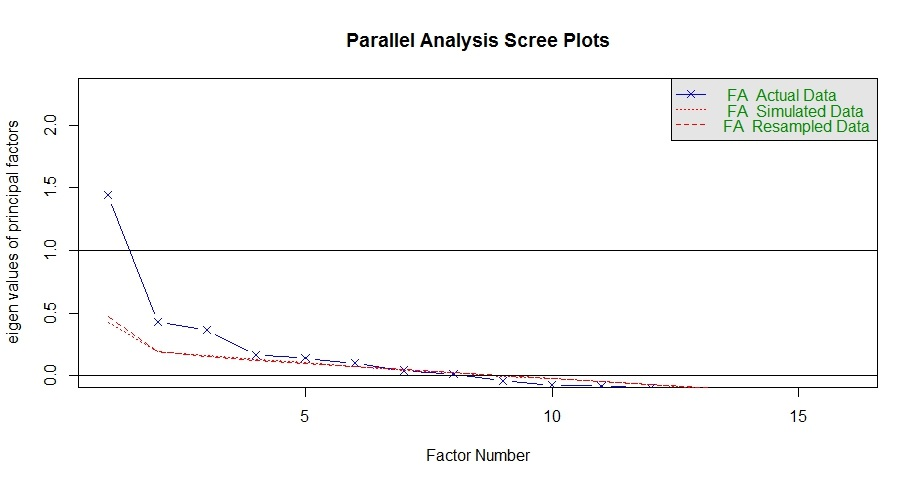
\includegraphics[width=\textwidth]{figs/PAonlyFA.jpg}
  \caption{Parallel analysis approach scree plote\label{fig:PAonlyFA}}
 \end{figure}

While the results from the exploratory analysis suggest that there may be multiple dimensions that underlie the FM LP assessment, the results need to be interpreted with caution. Note that, in practice, it is unlikely any empirical data will be purely unidimensional. That is, data may be considered basically as unidimensional when it has a "dominant" factor underlying the responses (e.g., \cite{Lord,1980})where any other factors can be thought as nuisance dimensions.  \footnote{Remember that an eigenvalue represent the amount of the information captured by a factor, and the first factor in Figure ~\ref{fig:PAonlyFA} has the value of 1.44, which is pretty small in comparison to values we observe in most testing situations.} 


I also will discuss a few examples based on the simulated data, and so that I will include the R code for the interested reader (R Development Core Team, 2010).

set.seed(12344321)
\begin{lstlisting}[language=R]
	 rasch.sim         <- function( nitem = 20, npers = 100 ) {
    i.loc         <- rnorm( nitem )
    p.loc         <- rnorm( npers ) 
    temp          <- matrix( rep( p.loc, length( i.loc ) )
                        , ncol = length( i.loc ) )
    logits        <- t( apply( temp, 1, '-', i.loc) )
    probabilities <- 1 / ( 1 + exp( -logits ) )
    resp.prob     <- matrix( probabilities, ncol = nitem)
    obs.resp      <- matrix( sapply( c(resp.prob), rbinom, n = 1, size = 1), 		 
    ncol = length(i.loc) )
    output        <- list()
    output\$i.loc  <- i.loc
    output\$p.loc  <- p.loc
    output\$resp   <- obs.resp
    output
}
\end{lstlisting}

\section {\em Attribute Hierarchy Model Results}

I used AHM to produce probabilities on each attribute for each student. I also examine the correlation among attributes to decide if the expected relationship is observed (i.e. high correlation between adjacent attributes). For placing a student into a mastery category for each attribute, I examined the results across three selected thresholds;0.75 which is highly conservative,0.65, and 0.50 which leads more students placed on mastery category of attributes. Table \ref{AHMcutoff} provides the mastery placement results into LP levels with these cutoffs. 

\begin{table}[htp]
\centering
\addtolength{\tabcolsep}{2pt} % some more room between columns
\caption{The distribution of levels with different cutoff values\label{table:AHMcutoff}}
\begin{tabular}{
 l
  S[table-format=2.0]
  S[table-format=2.1]
  S[table-format=1.1]
  S[table-format=-1.2]
  S[table-format=.2,table-comparator=true]
}
\toprule
{Cutoff} & {Attribute1} & {Attribute2} & {Attribut3} & {Attribute4} \\
\midrule
0.55 & 0.99 &0.75 &0.68 &0.66 \\
0.65 & 0.99 &0.69 &0.66 &0.55 \\
0.75 & 0.99 &0.62 &0.58 &0.30 \\

\midrule[\heavyrulewidth]
\end{tabular}
\end{table}

\subsection{AHM simulation}

To examine whether these results were unique to my data set, I simulated data from dichotomously scored items according to a five-attribute hierarchy with a simple conjunctive structure. The simulated data set had \textbf{HCI} distributions with means of about 0.60, and medians of 0.71. 

  
\begin{figure}[htbp]
  \centering
  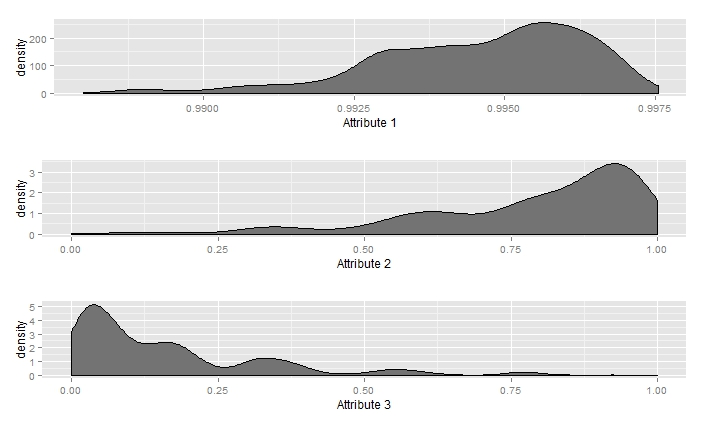
\includegraphics[width=\textwidth]{figs/AHM_simu.jpg}
  \caption{Averaged Attribute Estimates \label{fig:AHM_simu}}
 \end{figure}


My examination of the attribute estimates from an ANN resulted in similar findings.As it is seen in Figure \ref{figs/AHM_simu}I observed noticeable variation in attribute estimates in both simulated data sets after ensemble averaging, particularly for response patterns with HCI values lower than 0.7.

